\section*{\begin{tabular*}{\linewidth}{@{}l @{\extracolsep{\fill}} r@{}}
Nr.~15 & MUN~87/1 \\
\end{tabular*} 
}

\textsf{\textbf{Munda (Likwala-aux-Herbes; Fpl.~304)}}

\vspace{1em}

\noindent\begin{tabular}{@{}rl@{}}
	\textbf{Feldarbeit:} & \begin{tabular}[t]{@{}l@{}}\textbf{19.08.--30.08.1987}\\ \textbf{(M. K. H. Eggert)}\end{tabular} \\ 
	\textbf{Abb.:} & \textbf{\ref{fig:MUN87_Fundstelle}--\ref{fig:MUN87-1_14C-Kalibration}} \\ 
	\textbf{Tab.:} & \textbf{\ref{tab:MUN87-1_Konkordanz-Profile}--\ref{tab:MUN87-1_Funde}}\\
	\textbf{Taf.:} & \textbf{88.4--90.2} \\ 
	\textbf{Lit.:} & \textbf{--} \\ 
\end{tabular} 

\paragraph{Grabung und Befunde}\hspace{-.5em}|\hspace{.5em}%
In Munda am oberen \mbox{Likwala}-\mbox{aux}-\mbox{Herbes} wurde insgesamt vier Befunde untersucht (Abb.~\ref{fig:MUN87_Fundstelle}). Die beiden im Grabungsschnitt MUN~87/2 erfassten Inventare (Kat.-Nr.~16--17) wurden, zusammen mit dem aus der in Pikunda am \mbox{Sangha} ausgegrabenen Grube (Kat.-Nr.~8), für die Beschreibung der ältesten keramischen Stilgruppe im Arbeitsgebiet herangezogen.\footnote{Die entsprechende Keramik wurde erstmals von \textcites{Eggert.1992}{Eggert.1993} als Pikunda-Munda-Gruppe beschrieben (Kap.~\ref{sec:PKM-Gr}).} Die Grabung MUN~87/1 (Kat.~Nr.~15) erbrachte ein diagnostisches Inventar für den jüngeren, entlang des \mbox{Likwala}-\mbox{aux}-\mbox{Herbes} und \mbox{Sangha} verbreiteten Ebambe-Stil (Kap.~\ref{sec:EBA-Gr}). Etwa 7\,m südöstlich dieser Grabung fand sich ein weiterer kleiner Schlackenhügel sowie eine lange Tuyère (Abb.~\ref{fig:MUN87-101_Tuyere}).

\begin{figure*}[!tb]
 \centering
 \begin{subfigure}[t]{\columnwidth}
 \centering
 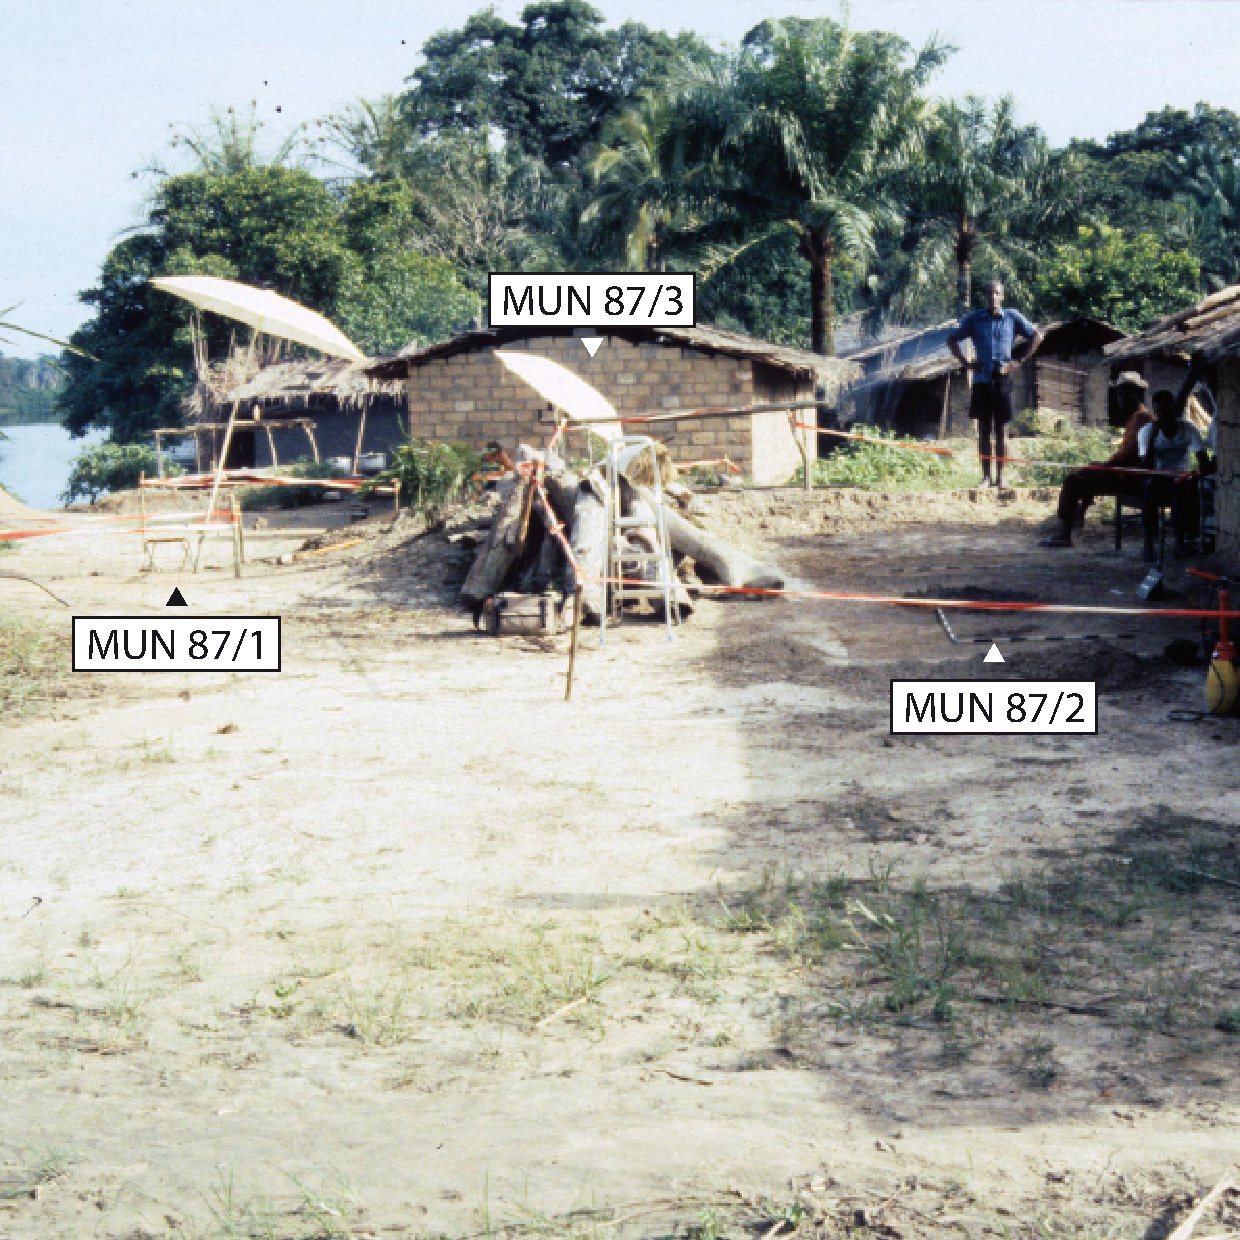
\includegraphics[width = \textwidth]{fig/MUN87_E87-038-31.pdf}
 \caption{Übersicht von Norden (Foto: M. K. H. Eggert, 1987).}
 \label{fig:MUN87_Übersicht1}
 \end{subfigure}\hfill
 \begin{subfigure}[t]{\columnwidth}
 \centering
 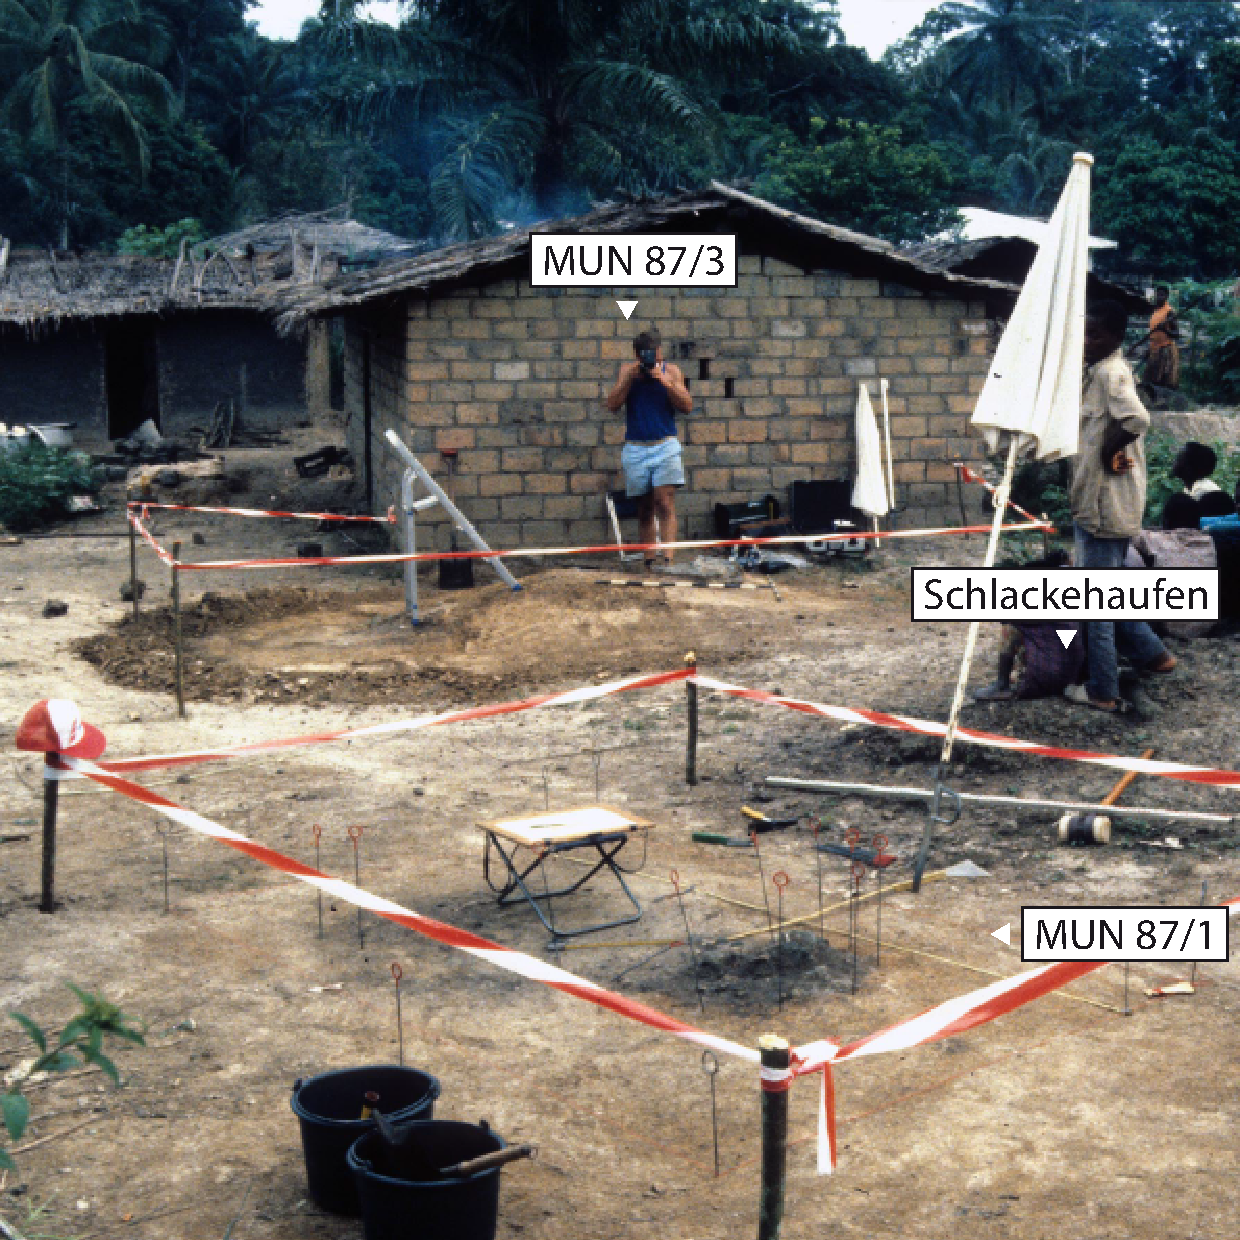
\includegraphics[width = \textwidth]{fig/MUN87_E87-038-36.pdf}
 \caption{Übersicht von Norden (Foto: M. K. H. Eggert, 1987).}
 \label{fig:MUN87_Übersicht2}
 \end{subfigure}\vspace{1em}
 \begin{subfigure}[t]{\columnwidth}
 \centering
 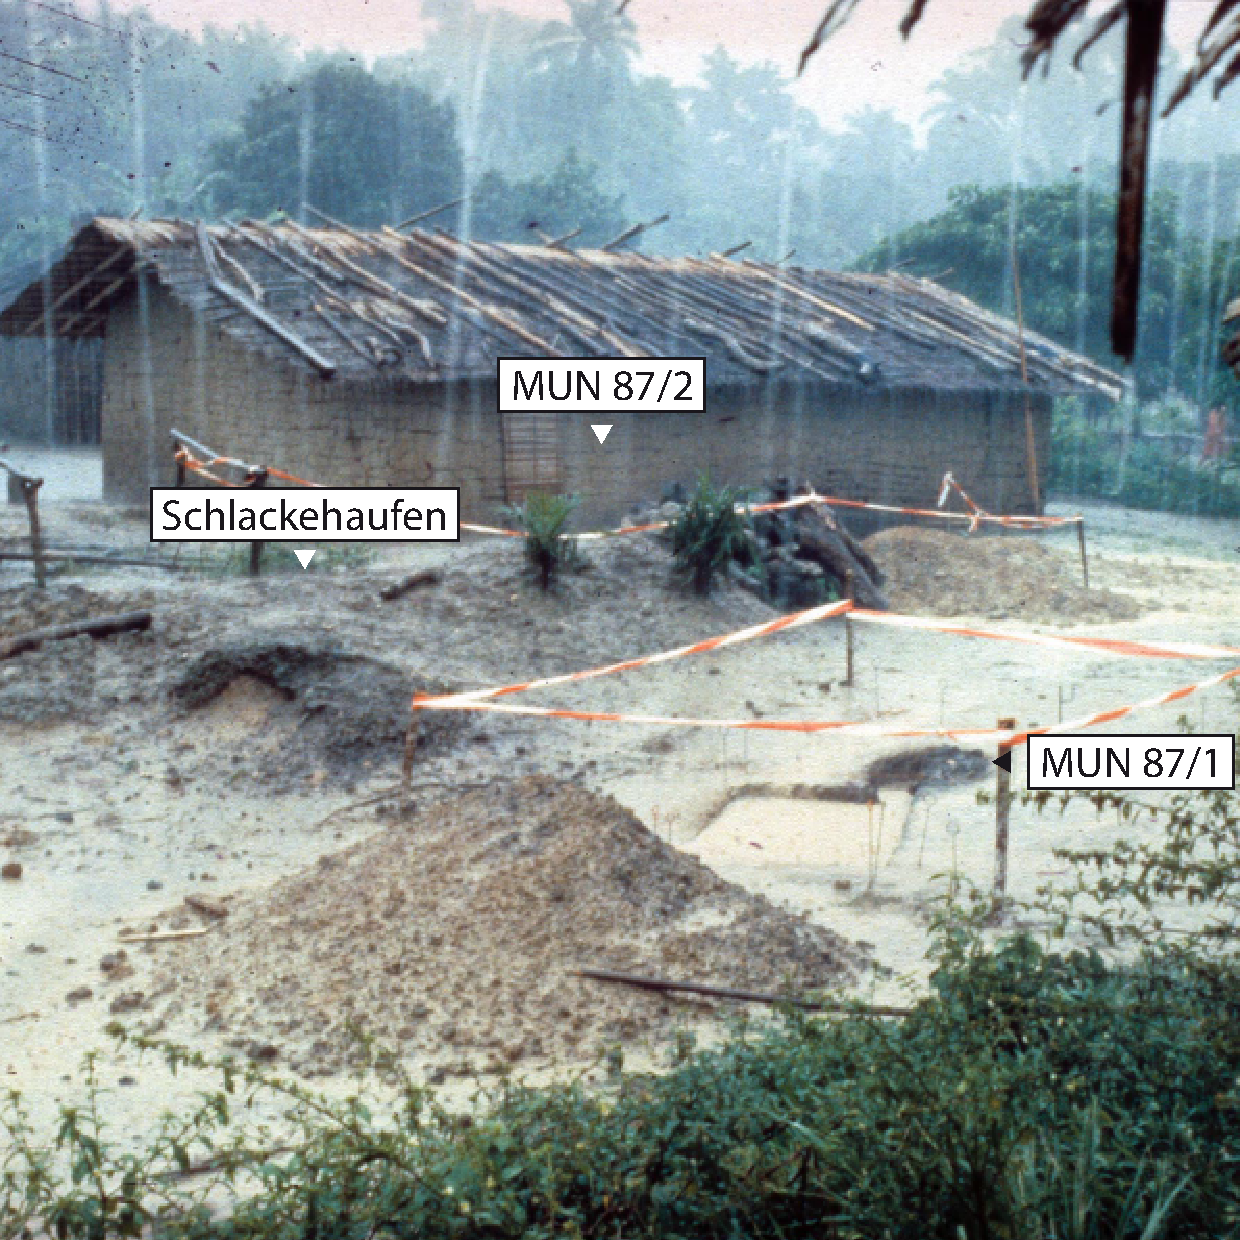
\includegraphics[width = \textwidth]{fig/MUN87_HH87-IV-9-II.pdf}
 \caption{Übersicht von Osten (OSO; Foto: H. Holsten, 1987).}
 \label{fig:MUN87_Übersicht3}
 \end{subfigure}\hfill
 \begin{subfigure}[t]{\columnwidth}
 \centering
 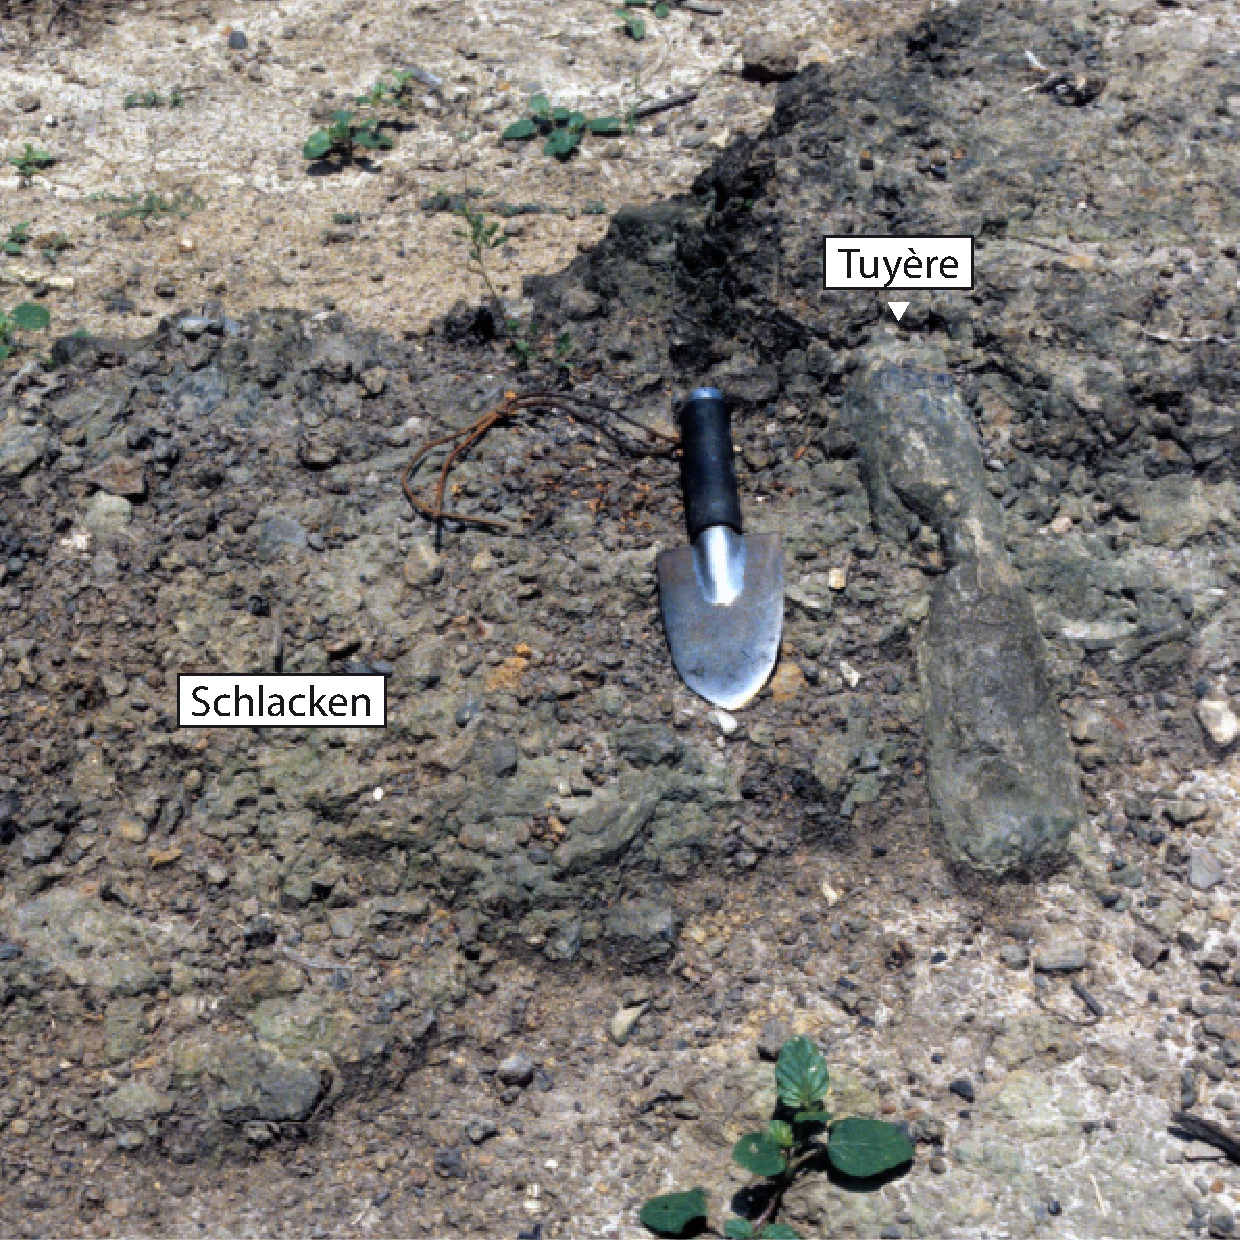
\includegraphics[width = \textwidth]{fig/MUN87-101_E87-035-35.pdf}
 \caption{Tuyère südöstlich von MUN~87/1 und östlich von MUN~87/3 (Foto: M. K. H. Eggert, 1987; siehe Abb.~\ref{fig:MUN87_Fundstelle}).}
 \label{fig:MUN87-101_Tuyere}
 \end{subfigure}
 \caption{Munda (Fpl.~304): Übersicht.}
 \label{fig:MUN87_Fundstelle_Fotos}
\end{figure*}

Die Grabung MUN~87/1 diente der näheren Untersuchung einer auffällig zweigeteilten Verfärbung (Abb.~\ref{fig:MUN87-1-0_Foto}--C). Diese bestand aus einer etwa 0,6\,m großen, stark mit gebrannten Lehmbrocken und Schlacke durchsetzten dunklen Verfärbung, dem späteren Befund MUN~87/1-0-1. An ihrem südöstlichen Ende schloss sich eine als MUN~87/1-0-2 bezeichnete größere, runde Verfärbung an (Abb.~\ref{fig:MUN87-1_Obfl_ZeichnungFoto}). Auf der Oberfläche lagen kleine Schlackebrocken, etwas unverzierte Keramik und gebrannte Tonbrocken, die eventuell zu einer Ofenwandung gehört haben könnten.

\begin{figure*}[p]
	\centering
	\begin{subfigure}[t]{0.32\textwidth}
		\centering
		\includegraphics[width = \textwidth]{fig/MUN87-1_1a.pdf}
		\caption{MUN~87/1: Zeichnung der \\Situation an der Oberfläche}
		\label{fig:MUN87-1-0_Zeichnung}
	\end{subfigure}\hfill
	\begin{subfigure}[t]{0.32\textwidth}
		\centering
		\includegraphics[width = \textwidth]{fig/MUN87-1-0_E87-038-20_kompr.pdf}
		\caption{MUN~87/1: Oberfläche nach dem ersten Putzen.}
		\label{fig:MUN87-1-0_Foto}
	\end{subfigure}\hfill
	\begin{subfigure}[t]{0.32\textwidth}
		\centering
		\includegraphics[width = \textwidth]{fig/MUN87-1-0-1-0_E87-038-26_kompr.pdf}
		\caption{MUN~87/1-0-1: Oberfläche nach dem ersten Putzen.}
		\label{fig:MUN87-1-0-1-0_Foto}
	\end{subfigure}
	\caption{MUN~87/1: Situation bei der Auffindung des Befundes (Fotos: M. K. H. Eggert, 1987).}
	\label{fig:MUN87-1_Obfl_ZeichnungFoto}
\end{figure*}

\begin{figure*}[p]
	\centering
	\begin{subfigure}[t]{0.32\textwidth}
		\centering
		\includegraphics[width = \textwidth]{fig/MUN87-102_Pl1_E87-040-6.jpg}
		\caption{Planum 1: 0,1\,m unter Obfl.}
		\label{fig:MUN87-1-0-2_Pl_1}
	\end{subfigure}\hfill
	\begin{subfigure}[t]{0.32\textwidth}
		\centering
		\includegraphics[width = \textwidth]{fig/MUN87-102_Pl3_E87-040-36.jpg}
		\caption{Planum 3: 0,3\,m unter Obfl.}
		\label{fig:MUN87-1-0-2_Pl_3}
	\end{subfigure}\hfill
	\begin{subfigure}[t]{0.32\textwidth}
		\centering
		\includegraphics[width = \textwidth]{fig/MUN87-102_Pl4_E87-041-13.jpg}
		\caption{Planum 4: 0,4\,m unter Obfl.}
		\label{fig:MUN87-1-0-2_Pl_4}
	\end{subfigure}
	\begin{subfigure}[t]{0.32\textwidth}
		\centering
		\includegraphics[width = \textwidth]{fig/MUN87-102_Pl5_E87-041-33.jpg}
		\caption{Planum 5: 0,5\,m unter Obfl.}
		\label{fig:MUN87-1-0-2_Pl_5}
	\end{subfigure}\hfill
	\begin{subfigure}[t]{0.32\textwidth}
		\centering
		\includegraphics[width = \textwidth]{fig/MUN87-102_Pl6_E87-042-8.jpg}
		\caption{Planum 6: 0,6\,m unter Obfl.}
		\label{fig:MUN87-1-0-2_Pl_6}
	\end{subfigure}\hfill
	\begin{subfigure}[t]{0.32\textwidth}
		\centering
		\includegraphics[width = \textwidth]{fig/MUN87-102_Pl7_E87-042-20.jpg}
		\caption{Planum 7: 0,87\,m unter Obfl.}
		\label{fig:MUN87-1-0-2_Pl_7}
	\end{subfigure}
	\caption{MUN~87/1-0-2: Plana (Fotos: M. K. H. Eggert, 1987).}
	\label{fig:MUN87-1-0-2_PlanaFotos}
\end{figure*}

Der nordwestliche, kleinere Befund MUN~87/1-0-1 wurde entlang einer nordwestlich-südöstlich verlaufenden Profilachse geschnitten, die beide Bereiche in ihrer längsten Ausdehnung erfasst. Nur der südwestliche Teil des Befundes wurde ausgegraben. Bei etwa 0,2\,m unter der Oberfläche wurden die Funde getrennt, ein Planum wurde nicht angelegt. Die Eingrabung reicht insgesamt bis in eine Tiefe von etwa 0,4\,m unter die rezente Oberfläche. Innerhalb der Verfüllung fanden sich durchgehend kleine Schlackebrocken (Abb.~\ref{fig:MUN87-1_VerteilungFunde}). Eine dezidierte Ofenwandung ließ sich nicht erkennen. Vielmehr fanden sich gelegentlich einzelne mehr oder weniger flache gebrannte Tonbrocken (Abb.~\ref{fig:MUN87-1_Ofenwand}). Ab etwa 0,1\,m unter der Oberfläche war die Verfüllung verstärkt mit Holzkohle durchsetzt. Das Sediment ist in einer zirka 0,1\,m breiten Zone um den Befund herum rötlich verziegelt (Abb.~\ref{fig:MUN87-1-0-1-0_Foto}). Dieser Bereich geht sukzessive in den anstehenden gelben Lehm über. Im nördlichen Teil des Befundes fand sich ab 0,25\,m unter der Oberfläche ein großer Block grünliche Fließschlacke sowie viele größere grünlich Schlackebrocken (Abb.~\ref{fig:MUN87-1-0_Zeichnung}).

\begin{figure*}[p]
	\centering
	\begin{minipage}[b]{.3\textwidth}
		\begin{subfigure}[t]{\textwidth}
			\centering
			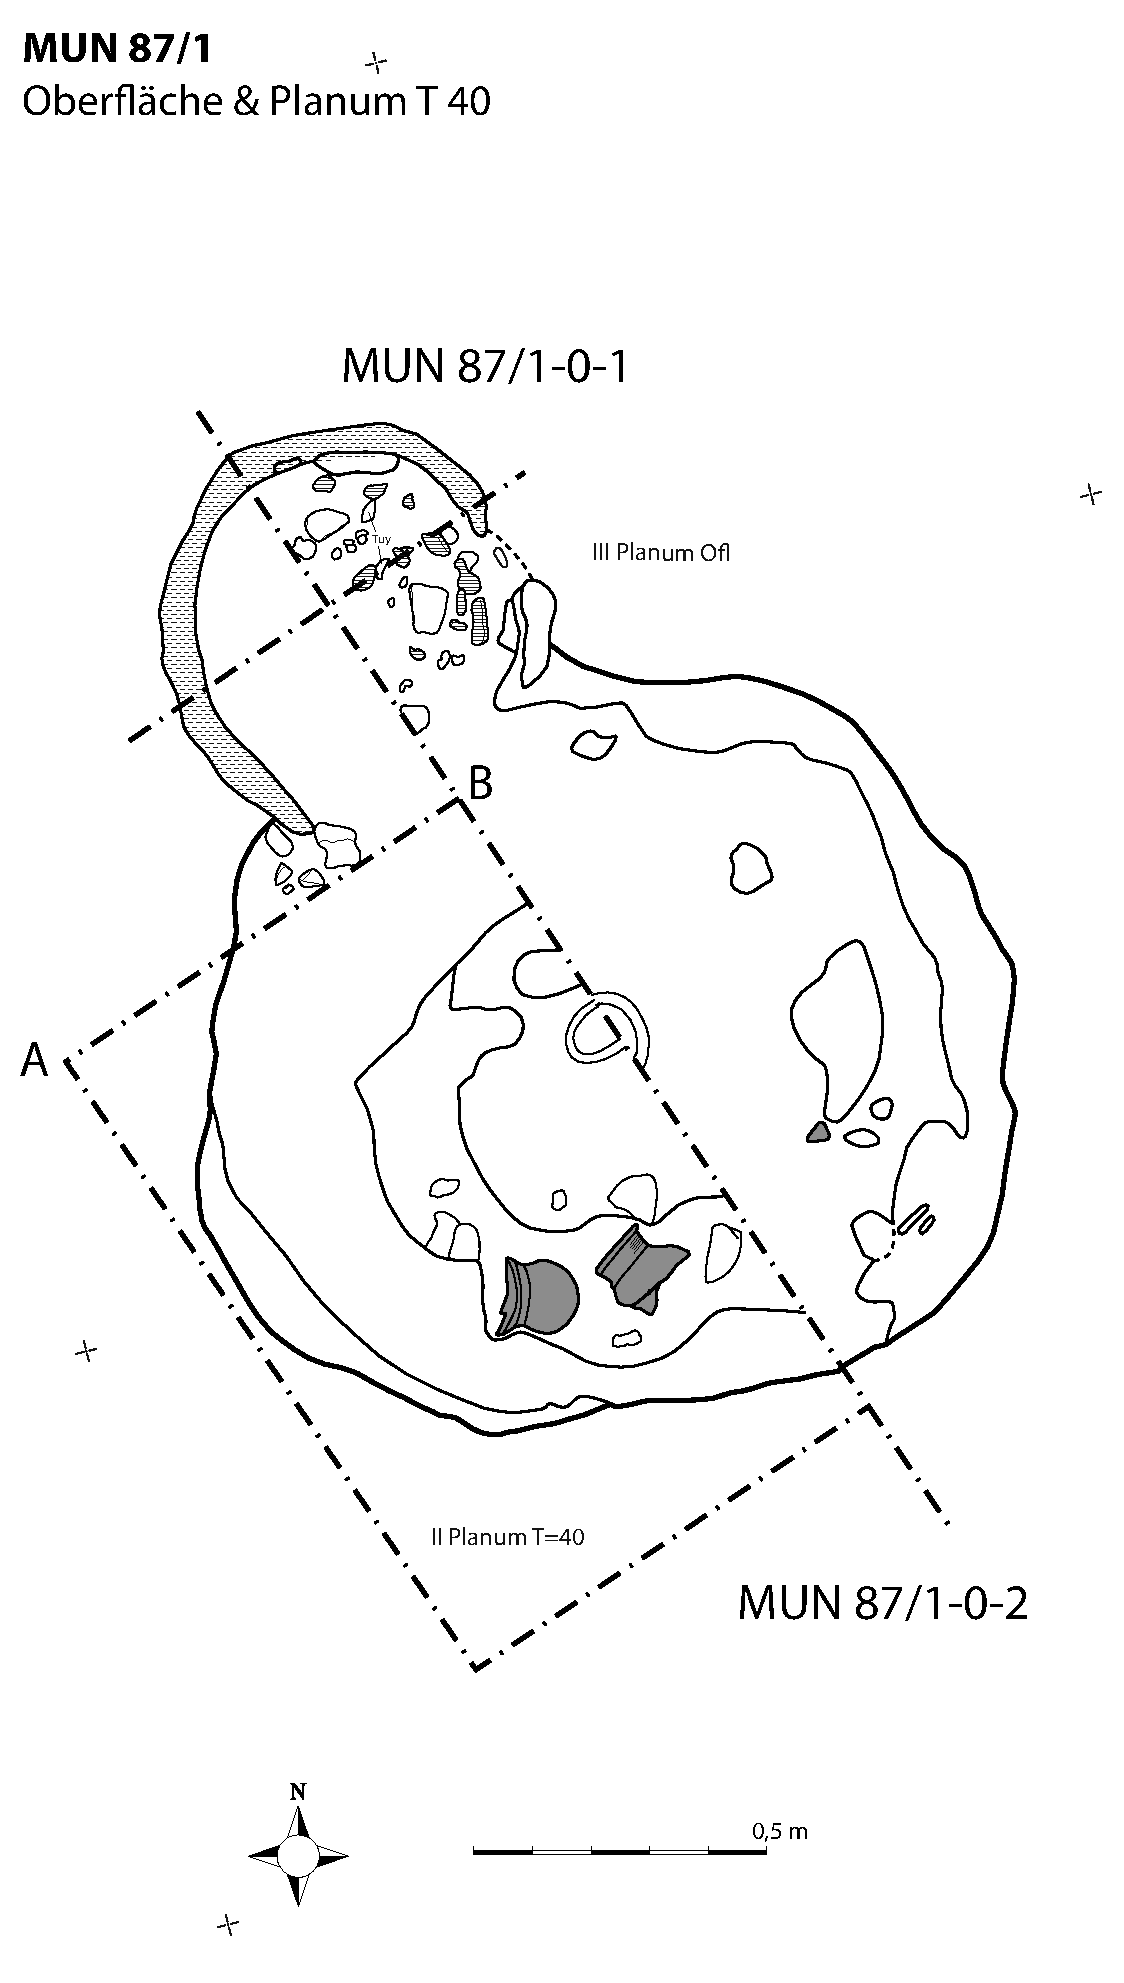
\includegraphics[width = \textwidth]{fig/MUN87-1_3Pl_T40Profil_A.pdf}
			\caption{Planum 2 (0,1\,m u. Obfl.).}
			\label{fig:MUN87-1_3Pl_T40Profil_A}
		\end{subfigure}
	\end{minipage}\hspace{1em}
	\begin{minipage}[b]{.55\textwidth}
		\begin{subfigure}[t]{.47\textwidth}
			\centering
			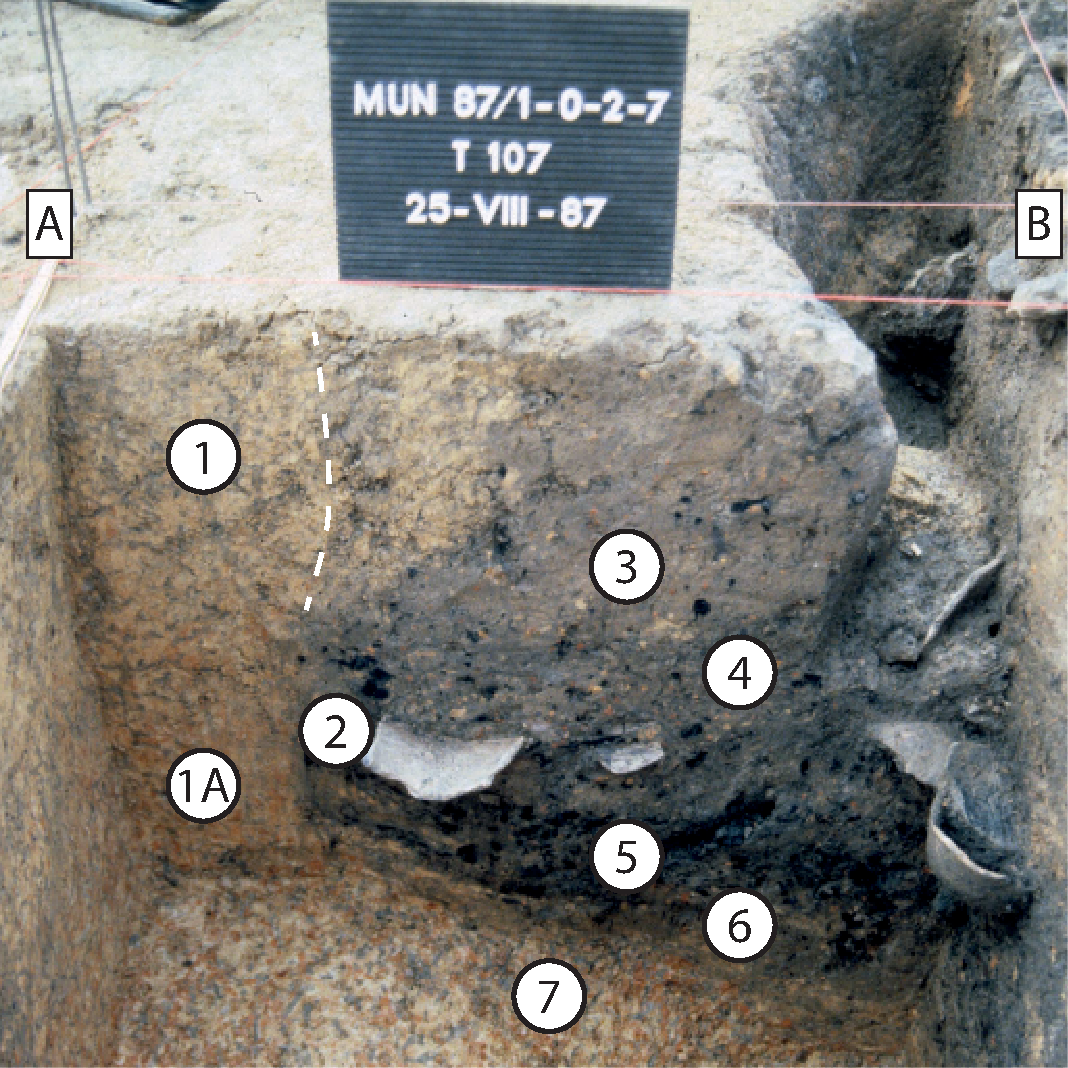
\includegraphics[width = \textwidth]{fig/MUN87-1_3Pl_T40Profil_B.pdf}
			\caption{Profil A--B.}
			\label{fig:MUN87-1_3Pl_T40Profil_B}
		\end{subfigure}\hspace{1em}%
		\begin{subfigure}[t]{.47\textwidth}
			\centering
			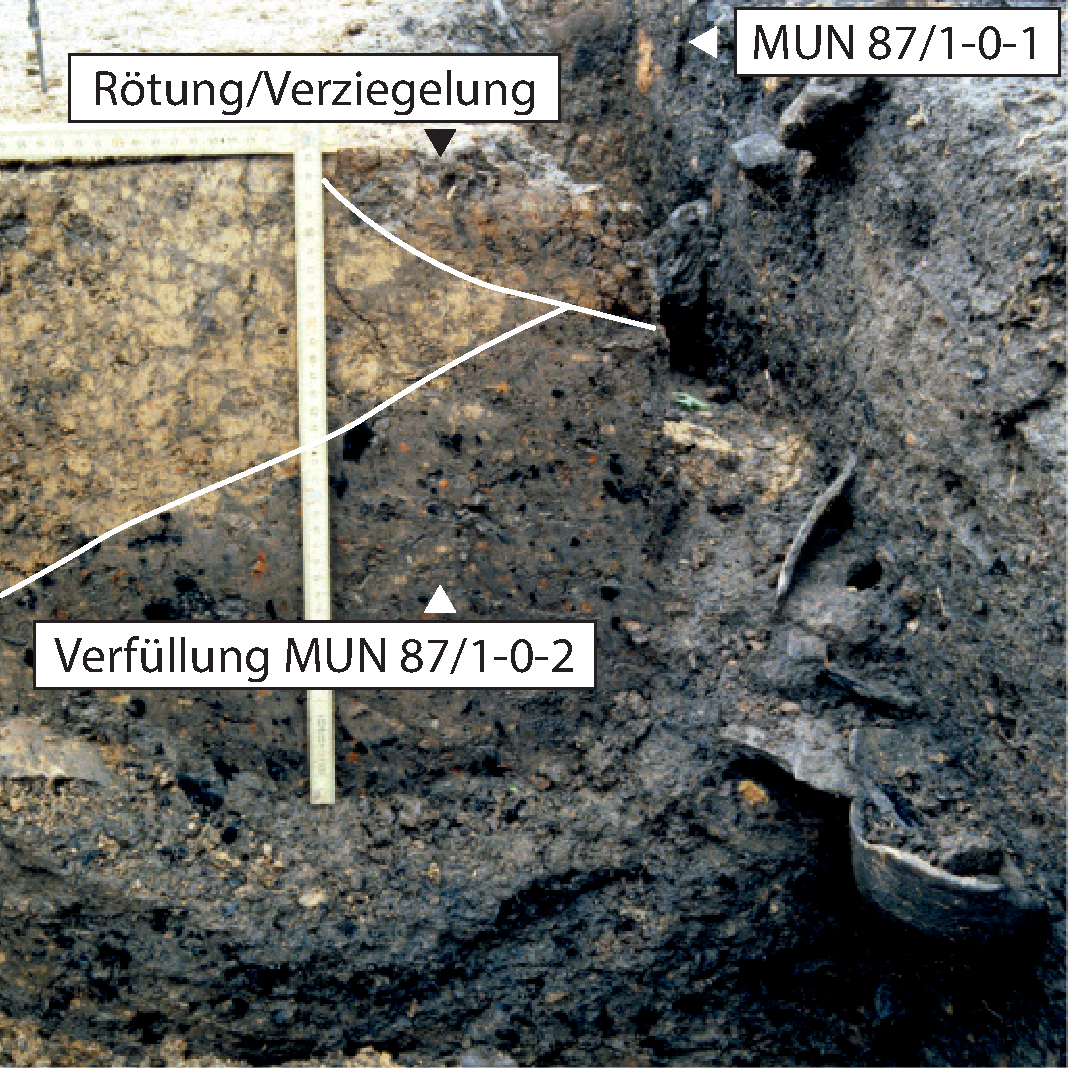
\includegraphics[width = \textwidth]{fig/MUN87-1_3Pl_T40Profil_C.pdf}
			\caption{Zurückverlegung Profil A--B.}
			\label{fig:MUN87-1_3Pl_T40Profil_C}
		\end{subfigure}
		\begin{subfigure}[t]{.47\textwidth}
			\centering
			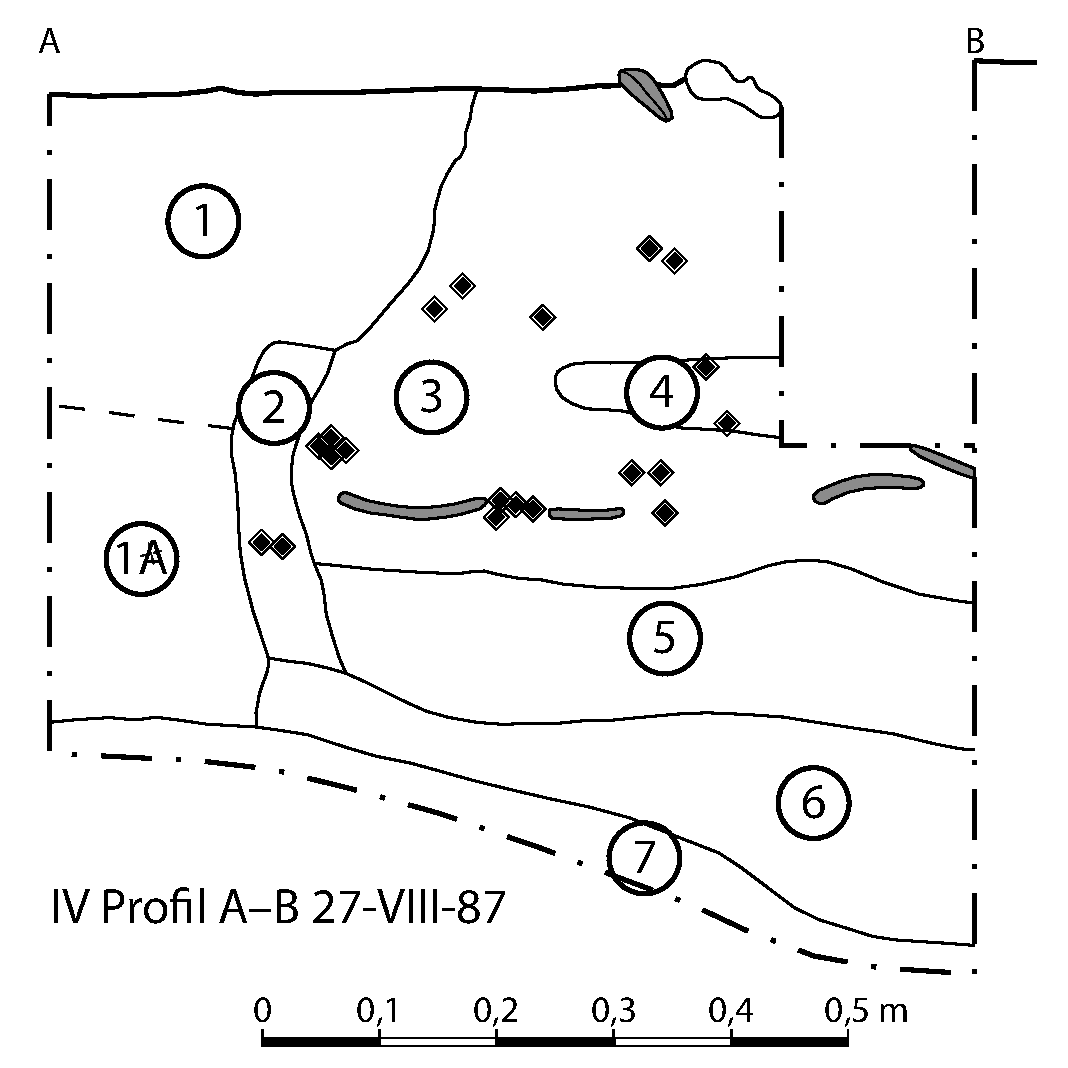
\includegraphics[width = \textwidth]{fig/MUN87-1_3Pl_T40Profil_D.pdf}
			\caption{Profil A--B.}
			\label{fig:MUN87-1_3Pl_T40Profil_D}
		\end{subfigure}\hspace{1em}%
		\begin{subfigure}[t]{.47\textwidth}
			\centering
			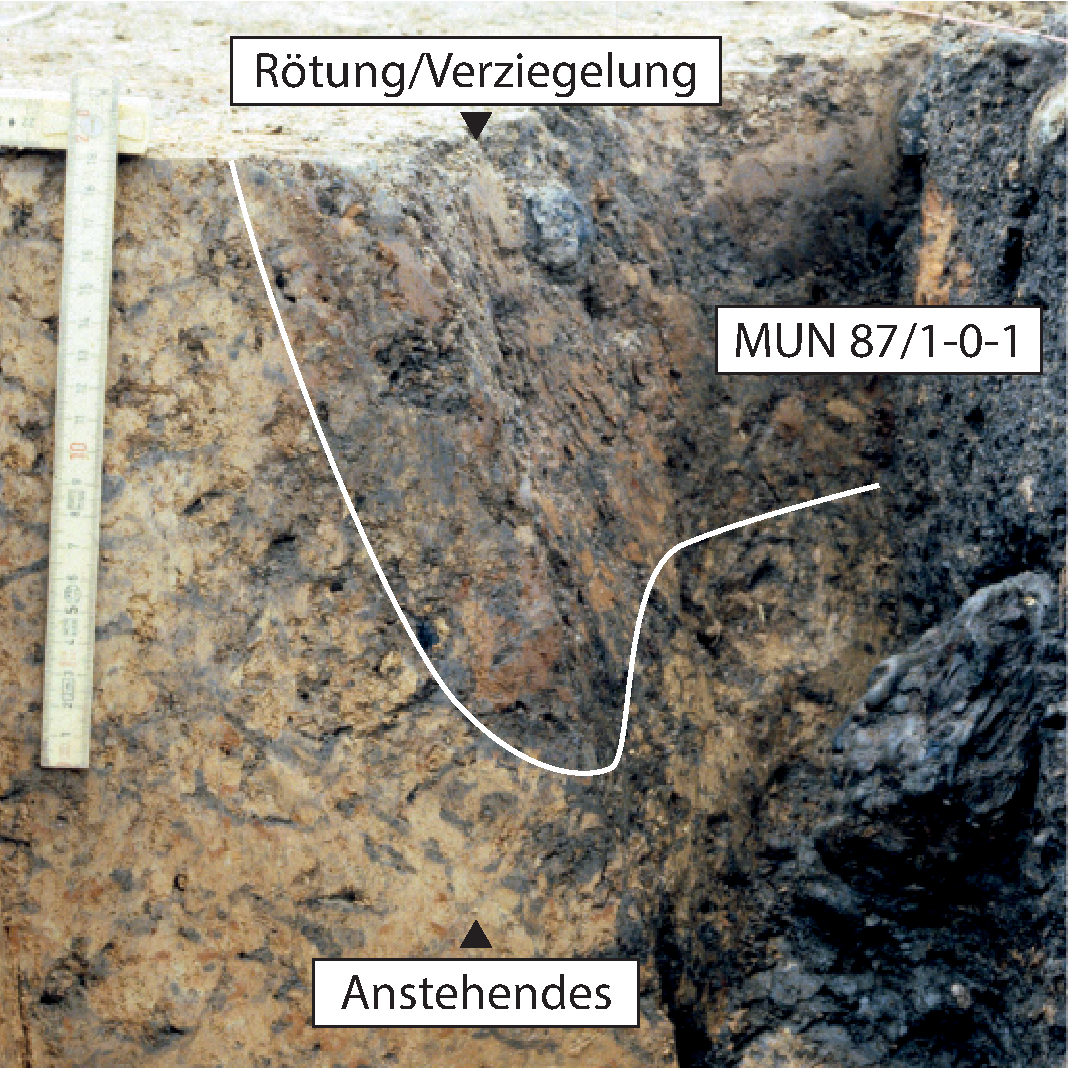
\includegraphics[width = \textwidth]{fig/MUN87-1_3Pl_T40Profil_E.pdf}
			\caption{Zurückverlegung Profil A--B.}
			\label{fig:MUN87-1_3Pl_T40Profil_E}
		\end{subfigure}	
	\end{minipage}
	\caption{MUN~87/1-0-2: Stratigrafische Relation zwischen Verhüttungsbefund MUN~87/1-0-1 und Grube MUN~87/1-0-2 (Fotos: M. K. H. Eggert, 1987).}
	\label{fig:MUN87-1_Querprofil_Zeichnung+Foto}
\end{figure*}

\begin{figure*}[p]
	\centering
	\begin{subfigure}[t]{.75\textwidth}
		\centering
		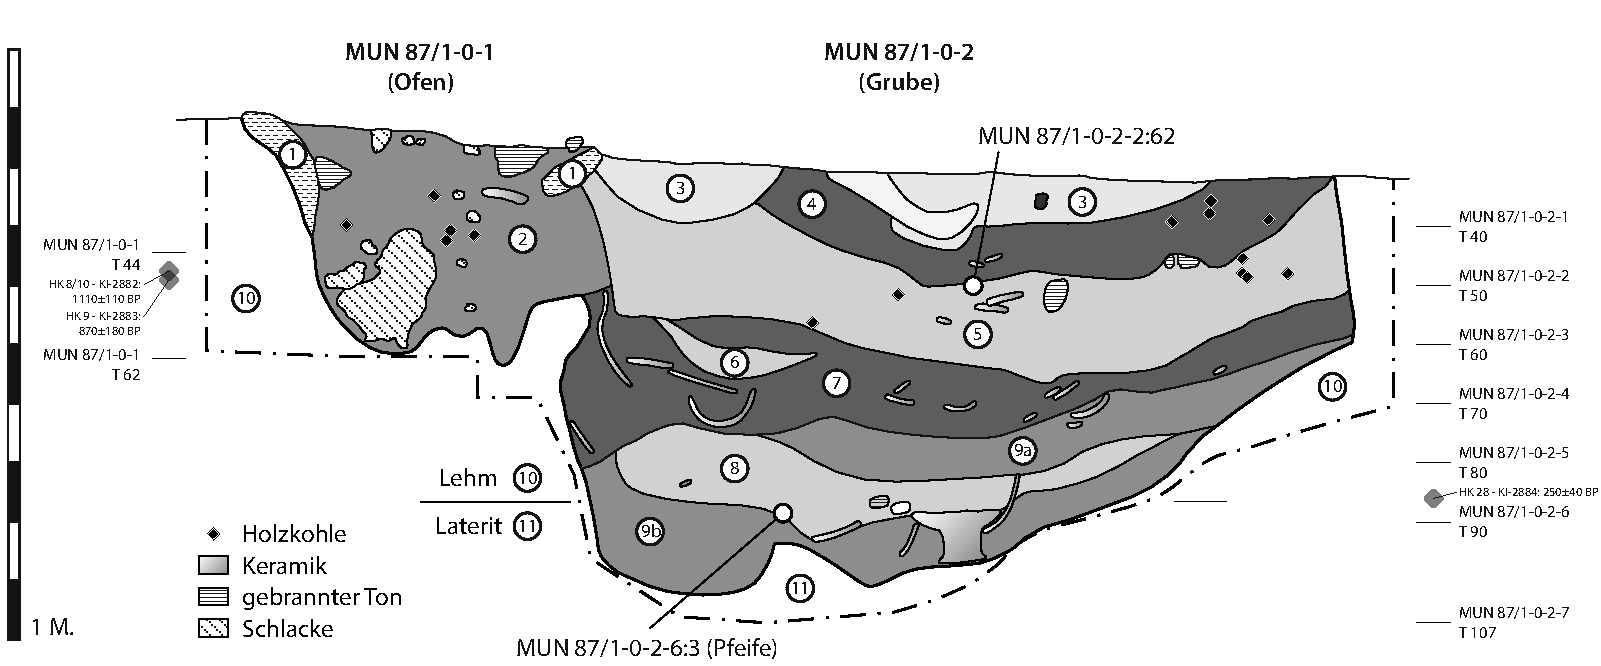
\includegraphics[width = \textwidth]{fig/MUN87-1_Profil_A.pdf}
		\caption{}
		\label{fig:MUN87-1_Profil_A}
	\end{subfigure}
	\begin{subfigure}[t]{.8\textwidth}
		\centering
		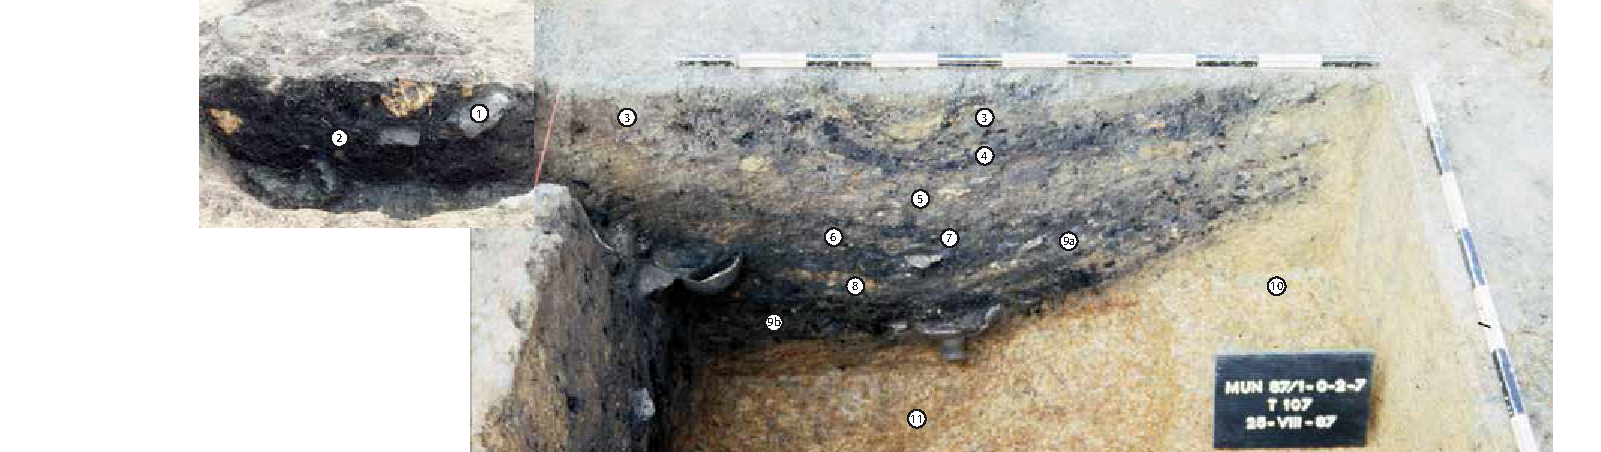
\includegraphics[width = \textwidth]{fig/MUN87-1_Profil_B.pdf}
		\caption{}
		\label{fig:MUN87-1_Profil_B}
	\end{subfigure}	
	\caption{MUN~87/1: Profil (Fotos: M. K. H. Eggert, 1987).}
	\label{fig:MUN87-1_Profil_Zeichnung}
\end{figure*}

\begin{table*}[p]
	\centering{\footnotesize\begin{sftabular}{@{}cc@{}}
			\toprule
			\textbf{Querprofil A--B} & \textbf{Längsprofil} \\ 
			\midrule
			1 & 10 \\ 
			5 & 4/7 \\ 
			6 & 9 \\ 
			7 & 11 \\ 
			\bottomrule
	\end{sftabular}} 
	\caption{MUN~87/1: Konkordanzliste für die Schicht-Nummerierung des Quer- (Abb.~\ref{fig:MUN87-1_3Pl_T40Profil_B}, \ref{fig:MUN87-1_3Pl_T40Profil_D}) und Längsprofils (Abb.~\ref{fig:MUN87-1_Profil_Zeichnung}).}
	\label{tab:MUN87-1_Konkordanz-Profile}
\end{table*}

Direkt anschließend an den kleineren Befund MUN~87/1-0-1 wurde eine knapp 0,7\,m tiefe Grube, die eine Durchmesser von etwa 1,4\,m aufwies, ausgegraben. Während vor der Oberfläche weniger Funde abgesammelt werden konnten, ließ sich nach dem groben Putzen eine auffällige Binnengliederung aus helleren und dunkleren Bereichen beobachten (Abb.~\ref{fig:MUN87-1-0_Foto}). Die Grube wurde entlang der Hauptprofilachse geschnitten (Abb.~\ref{fig:MUN87-1_Profil_Zeichnung}).\footnote{Die Grabung erfolgte in sieben künstlichen Abträgen. Mit Ausnahme einer zeichnerischen Dokumentation des ersten Planums bei etwa 0,1\,m unter der Oberfläche (Abb.~\ref{fig:MUN87-1_3Pl_T40Profil_A}) wurden die folgenden Plana lediglich fotografisch dokumentiert (Abb.~\ref{fig:MUN87-1-0-2_PlanaFotos}).} Bei etwa 0,5--0,6\,m unter der Oberfläche wurde das an Laterit reiche Anstehende erreicht (Abb.~\ref{fig:MUN87-1-0-2_Pl_6}, \ref{fig:MUN87-1_Profil_A}). Die Verfüllung besteht aus sich abwechselnden hellen und dunklen Schichten. Die Grenzen zwischen den einzelnen Lagen sind recht scharf ausgebildet. In den oberen 0,2--0,3\,m ist die Wandung der Grube gerade bis steilschräg und an einigen Stellen sogar leicht überkippt (Abb.~\ref{fig:MUN87-1_3Pl_T40Profil_B}--C), um dann mit einem auffällig scharfen Knick zur konvexen Grubensohle umzubrechen.

Der nordwestliche, in Richtung des Ofens liegende Teil der Grubenverfüllung war im ersten Abtrag sehr hart. Weiter unten ist dieser Teil der Grube mit teilweise recht großen Stücken Holzkohle durchsetzt gewesen. Ab dem dritten und vierten Abtrag, 0,2--0,4\,m unter der Oberfläche, zeigte sich im Bereich der Grubenwandung eine deutliche Konzentration von Holzkohle, welche die Wandung wie ein \textit{Gürtel} umschloss (Abb.~\ref{fig:MUN87-1-0-2_Pl_3}--C). Im fünften und sechsten Abtrag fanden sich jeweils ein großes Stück Ofenwandung, wie es auch im benachbarten Verhüttungsbefund MUN~87/1-0-1 zu finden war (Abb.~\ref{fig:MUN87-1_Ofenwand}).

Keramik fand sich in den oberen Plana vor allem im südlichen Teil der Grube (Abb.~\ref{fig:MUN87-1-0-2_Pl_1}--B). Das Inventar besteht aus -- in mehreren Lagen aufgefundenen -- großen Gefäßscherben und fast vollständigen Gefäßen. An der Sohle der Grube fand sich eine sehr fragmentierte aber vollständige Flasche mit stark geschweifter Wandung und kurzem Kegelhals (Abb.~\ref{fig:MUN87-1-0-2_Pl_6}; Taf.~90.2). Zwischen den Fragmenten dieser Flasche fanden sich kleine Knochenreste, die allerdings nicht geborgen wurden. Unter der zerscherbten Flasche wurde noch eine potenziell aus lokaler Produktion stammende tönerne Pfeife gefunden (Kap.~\ref{sec:Pfeifen}; Taf.~88.9). 

Der stratigrafische Zusammenhang zwischen der potenziell als Verhüttungsbefund ansprechbaren Struktur MUN~87/1-0-1 zur direkt anschließenden größeren Grube MUN~87/1-0-2 sollte durch ein Querprofil zweifelsfrei abgeklärt werden (Abb.~\ref{fig:MUN87-1_Querprofil_Zeichnung+Foto}). Ein erster Profilkasten, der von der ausgenommenen Verfüllung des Befundes MUN~87/1-0-1 in Richtung Südwest-Nordost ausging, erbrachte kein Ergebnis. Durch mehrfaches Rückverlegen des Profils A--B konnte beobachtet werden, dass die rote, mit Befund MUN~87/1-0-1 zu assoziierende Verziegelung die Verfüllung der Grube überlagert. Demnach wäre der Befund MUN~87/1-0-1, der kleine Ofen, stratigraphisch jünger als die Grube MUN~87/1-0-2 (Abb.~\ref{fig:MUN87-1_3Pl_T40Profil_C}). Dieser Befund lässt sich jedoch weder durch die Radiokohlenstoffdatierungen (Abb.~\ref{fig:MUN87-1_14C-Kalibration}; Tab.~\ref{tab:MUN87-1_14C-Daten}), noch die Fundauswertung bekräftigen.

\begin{table*}[tb]
	\centering{\footnotesize
		\begin{sftabular}{@{}lrrrr@{}}
\toprule
\textbf{Fundkategorie} &  \textbf{Anzahl} &    \textbf{\%} &  \textbf{Gewicht (kg)} &   \textbf{\%} \\
\midrule
        Eisen &       1 &   0,1 &          0,00 &   0,0 \\
      Keramik &     406 &  52,6 &         12,55 &  57,0 \\
     Ofenwand &      23 &   3,0 &          1,55 &   7,1 \\
     Schlacke &     332 &  43,0 &          7,66 &  34,8 \\
       Sonder &       3 &   0,4 &          0,15 &   0,7 \\
       Tuyere &       7 &   0,9 &          0,11 &   0,5 \\
\bottomrule
\end{sftabular}
 }
	\caption{MUN~87/1: Anteil verschiedener Fundmaterialien.}
	\label{tab:MUN87-1_Funde}
\end{table*}

\begin{figure*}[tb]
	\centering
	\includegraphics[width=\textwidth]{fig/9-12_MUN87-1_Fragmentierung_2.pdf}
	\caption{MUN~87/1: Fragmentierungsgrad der Scherben (n~=~406; Größenklassen siehe Anm.~\ref{ftn:Keramik_Fragmentierung}).}
	\label{fig:MUN87-1_Fragmentierung}
\end{figure*}

\vspace{1em}
\noindent Das Querprofil A--B erbrachte den folgenden stratigrafischen Befund (Abb.~\ref{fig:MUN87-1_3Pl_T40Profil_B} \& D):
\begin{itemize}[leftmargin=*, labelindent=1.25em, noitemsep, topsep=0pt]
	\item[(1)] anstehender gelber Lehm
	\item[(1A)] wie (1) aber fleckig rot: 2.5YR 4/8; Grenze zwischen (1) und (1A) fließend, leichte Lateritisierung
	\item[(2)] Mischzone zwischen (1)/(1A) \& (3), mit  Holzkohle durchsetzt
	\item[(3)] 10YR 3.5/5; mit etwas Holzkohle und kleinen, etwa 1\,cm großen rotverziegelten Brocken
	\item[(4)] 10YR 4/2 bis 2.5Y 3.5/2; mit relativ viel Holzkohle und kleinen rotverziegelten Partikeln
	\item[(5)] 2.5Y 3.5/2 bis 5Y 3.5/1; mit extrem viel Holzkohle
	\item[(6)] 10YR 4.5/2 bis Mischung aus 2.5Y 4/2 \& 10YR 4/2; westl./in Richtung (1) \& (1A) heller; wenig HK
	\item[(7)] wie (1A); aber \textit{lateritisiert}
\end{itemize}

\vspace{1em}
\noindent Das Längsprofil erbrachte den folgenden stratigrafischen Befund (Abb.~\ref{fig:MUN87-1_Profil_Zeichnung}):
\begin{itemize}[leftmargin=*, labelindent=1.25em, noitemsep, topsep=0pt]
	\item[(1)] 5YR 4/4 bis 2.5YR 4/8; gebrannter Lehm; Teile der Ofenwand/-wanne
	\item[(2)] 10YR 3/2 bis 10YR 3/1.5 \& 2.5Y 3/2; Füllung des Ofens
	\item[(3)] 10 YR 3.5/2
	\item[(4)] 2.5 Y 2.5/0; stark mit Holzkohle durchsetzt
	\item[(5)] 10 YR 4/2.5
	\item[(6)] 10 YR 4.5/3.5 bis 5 Y 3/1.5 \& 2.5 Y 3/2 mit 7.5 YR 5/6
	\item[(7)] 5 Y 3.5/1; stark mit Holzkohle durchsetzt
	\item[(8)] 2.5 Y 3.5/2 bis 5 Y 3.5/1.5; stark mit Holzkohle durchsetzt
	\item[(9)] Mischzone, zwischen 7/8 \& 10
	\item[(10)] steriler Lehm
	\item[(11)] steriler Lehm mit beginnender Lateritisierung
\end{itemize}

\paragraph{Keramik\vspace{.5em}}\mbox{}\\
\begin{tabular}{@{}lrl@{}}
Ausgezählt: & 3689\,g & \\ 
Bearbeitet: & 8858\,g & (71\,\%) \\ 
Insgesamt: & 12547\,g & \\ 
\end{tabular} 

\vspace{1em}
\noindent Die beiden erfassten Befunde weisen ein deutlich unterschiedliches Fundinventar auf (Abb.~\ref{fig:MUN87-1_VerteilungFunde}). Während im Verhüttungsbefund (MUN~87/1-0-1) kaum Keramik (5\,\%), dafür aber sehr viel Schlacke (89\,\%) gefunden wurde, enthielt die Grube (MUN~87/1-0-2) kaum Schlacken (4\,\%) und vor allem Keramik (87\,\%). Etwa die Hälfte aller Scherben ist zwischen 30\,$\times$\,30--70\,$\times$\,70\,mm groß (Abb.~\ref{fig:MUN87-1_Fragmentierung}). Jedoch umfasst das Inventar der Grube auch einen auffällig hohen Anteil großer Gefäßfragmente und vollständiger Gefäße (siehe Abb.~\ref{fig:MUN87-1-0-2_PlanaFotos}). 

\begin{figure*}[p]
	\centering
	\begin{subfigure}{\textwidth}	
		\centering
		\includegraphics[width = \textwidth]{fig/9-12_MUN87-1_VerteilungFunde_R.pdf}
		\caption{Fundmaterial\vspace{1em}}	
		\label{fig:MUN87-1_VerteilungFunde}
	\end{subfigure}
	\begin{subfigure}{\textwidth}
		\centering
		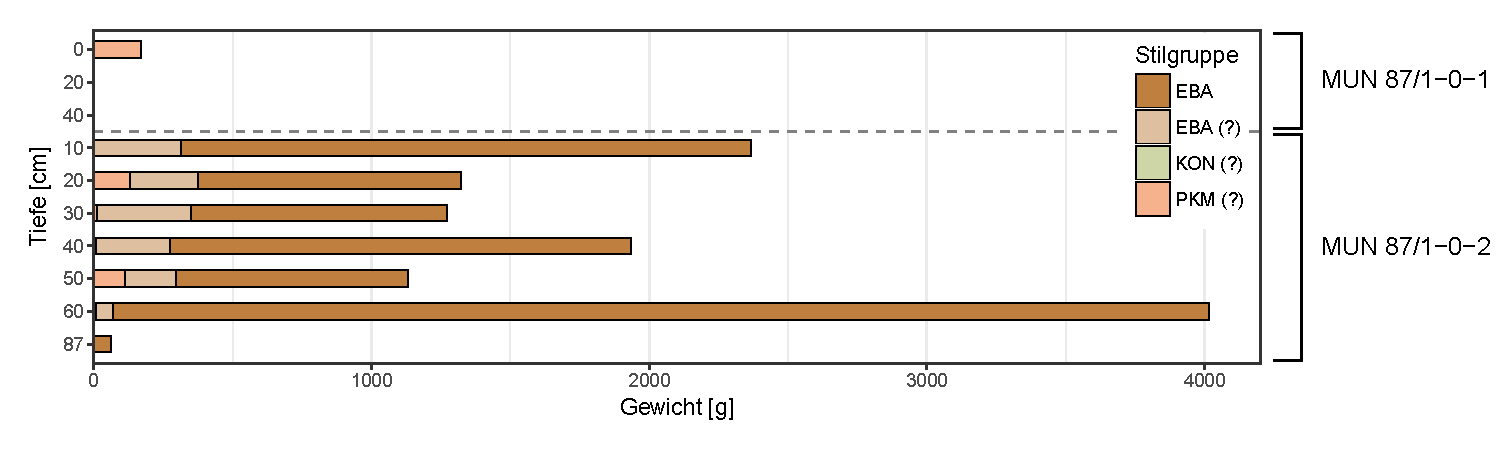
\includegraphics[width = \textwidth]{fig/9-12_MUN87-1_KeramikStilgruppen_R.pdf}
		\caption{Keramische Stilgruppen\vspace{1em}}
		\label{fig:MUN87-1_VerteilungStilgr}
	\end{subfigure}
	\begin{subfigure}{\textwidth}	
		\centering
		\includegraphics[width = \textwidth]{fig/9-12_MUN87-1_Fabrics_R.pdf}
		\caption{\textit{Fabrics}\vspace{1em}}
		\label{fig:MUN87-12_VerteilungFabrics}
	\end{subfigure}
	\begin{subfigure}{\textwidth}	
	\centering
		\includegraphics[width = \textwidth]{fig/9-12_MUN87-1_Schlacken_R.pdf}
		\caption{\textit{Schlacken}}
		\label{fig:MUN87-12_Schlacken}
	\end{subfigure}
	\caption{MUN~87/1: Verteilung der Fundmaterialien (A), keramischen Stilgruppen (B), \textit{Fabrics} (C) und Schlacken (D) in den entsprechenden Tiefen der Grabung.}
	\label{fig:MUN87-1_Funde}
\end{figure*}

Der Verhüttungsbefund (MUN~87/1-0-1) enthielt insgesamt nur sehr wenig Keramik (409\,g; Abb.~\ref{fig:MUN87-1_Funde}). Das Inventar unterscheidet sich deutlich von jenem aus der benachbarten Grube (MUN~87/1-0-2). Es enthält keine der für den Ebambe-Stil (Kap.~\ref{sec:EBA-Gr}) typischen Formen. Die einzige diagnostische Scherbe ist ein Randstück, das an die Ränder der Schalen des Pikunda-Munda-Stils erinnert (Kap.~\ref{sec:PKM-Gr}).\footnote{Das Stück weist einen kurzen, konkav ausbiegenden Rand auf, der ohne ausgebildeten Hals oder Schulterbereich direkt in die Gefäßwandung übergeht. Knapp unter dem Randabschluss sind noch Reste eines umlaufenden Bandes aus Wiegebandverzierung erhalten (Tab.~\ref{tab:Verzierungselemente}: 04.2). Sechs weitere, unverzierte Wandungsscherben ähneln technisch der Randscherbe so stark, das sie gemeinsam zu einer GE gehören könnten. Sie lassen sich jedoch aufgrund der starken Erosion der Bruchkanten nicht zusammensetzen.} Die besten Entsprechungen für das keramische Inventar finden sich im Fundgut des benachbarten Verhüttungsbefundes MUN~87/3 (Kat.-Nr.~18), welches der Pikunda-Munda-Gruppe zuzuordnen ist. 

Die Grube (MUN~87/1-0-2) enthielt ein sehr homogenes keramisches Inventar, das maßgeblich für die Beschreibung des Ebambe-Stils ist (Kap.\ref{sec:EBA-Gr}).\footnote{Die Scherben sind fast durchweg dem \textit{Fabric} 1 zuzuordnen und nur wenige Stücke weisen auf die Nutzung rotbrennender Tone hin (\textit{Fabric} 2; Abb.~\ref{fig:MUN87-12_VerteilungFabrics}).} Der Großteil der GE (86\,\%) kann sicher dem Ebambe-Stil zugewiesen werden (Abb.~\ref{fig:MUN87-1_VerteilungStilgr}).\footnote{Ein kleiner Anteil der Scherben (5\,\%) weist \textit{banfwa-nfwa}-Verzierung auf. Diese ist eines der diagnostischen Merkmale für den Ebambe-Stil (Kap.~\ref{sec:EBA-Gr}). Die wenigen nicht diagnostischen Scherben (8\,\%) weisen durchweg einen Scherben auf, der sich dem \textit{Fabric} 1 oder 2 zuordnen lässt.} In der Grube fanden sich einzelne Scherben, die potenziell dem Pikunda-Munda-Stil (Kap.~\ref{sec:PKM-Gr}) zugewiesen werden können (Taf.~88.4, 88.6).\footnote{Entsprechende Formen fanden sich im direkt an die Grube anschließenden Verhüttungsbefund (MUN~87/1-0-1). Eines dieser, nur schwerlich dem Ebambe-Stil zuweisbaren Stücke ist ein unverziertes, leicht bauchiges Gefäß mit Zylinderhals (Taf.~88.4).}

Das keramische Fundgut aus der Grube besteht vor allem aus hohen, leicht bauchigen Gefäßen mit Schulterabsatz und Kegel- oder Zylinderhals (Taf.~89). Während die Ränder dieser Gefäße regelhaft unverziert sind, sind Hals- und vor allem Schulterbereiche häufig verziert. In der Regel weisen die Zylinder- oder Kegelhälse eine aus horizontalen Rillen (Tab.~\ref{tab:Verzierungselemente}: 02.1), \textit{banfwa-nfwa} (Tab.~\ref{tab:Verzierungselemente}: 08) oder geritzten Kreuzmustern (Tab.~\ref{tab:Verzierungselemente}: 01.11) bestehende Verzierung auf. Die häufig schmale, getreppte Schulterpartie zeigt wiederholt einfache, diagonale Eindruckreihen auf, die mit einem kantigen oder seltener runden (04.11--12) Werkzeug erzeugt wurden. Die Wandungen und Gefäßunterteile sind fast durchweg mit großflächigem \textit{banfwa-nfwa} (Tab.~\ref{tab:Verzierungselemente}: 08) verziert. In keinem Fall ließ sich eine Verzierung der Standflächen beobachten, jedoch reicht die \textit{banfwa-nfwa}-Verzierung häufig direkt bis an den Bodenansatz hinunter.\footnote{Etwa 10\,\% der Scherben, fast ausschließlich Kegelhalsgefäße des Typs B4, weisen Reste organischer Anhaftungen auf. In den anderen, am Fundplatz untersuchten Gruben (Kat.-Nr.~16--17) lassen sich Anhaftungen nur sehr selten und an wenigen Einzelstücken beobachten. Bei den Anhaftungen handelt es sich entweder um glänzende, ölige Schichten an der Außenseite der Gefäße oder matte, bis zu 1\,mm dicke Krusten an den Gefäßinnenseiten.} Daneben finden sich noch einige Flaschen mit geschweifter Wandung und kurzem Kegelhals (Typ A2; Taf.~90), sowie kleine Schalen mit einem auffälligen Knick im Profil (Typ G4--5).\footnote{Eine fast vollständig erhaltene Schale weist einen hohen Standringboden auf (Taf.~88.8). Bei einem weiteren Fragment ist noch der Ansatz eines Standringbodens erhalten. Während einige der Schalen \textit{banfwa-nfwa}-Verzierung aufweisen, beschränkt sich die Verzierung größtenteils auf mit Ritzlinien gefüllte, gegenläufige Dreiecksflächen (Tab.~\ref{tab:Verzierungselemente}: 01.8; Taf.~88.8), eingeritzte Kreuzmuster (Tab.~\ref{tab:Verzierungselemente}: 01.11) oder breite Winkelbänder (Tab.~\ref{tab:Verzierungselemente}: 02.4) auf dem Rand oder Oberteil.} 

Die beobachteten Unterschiede zwischen dem Inventar des Verhüttungsbefundes (MUN~87/1-0-1) und dem der Grube (MUN~87/1-0-2) lassen sich potenziell mit dem funktionalen Charakter der jeweiligen Eingrabungen erklären. Gerade die dichten Packungen aus vollständigen Gefäßen oder großen Gefäßfragmenten in der Grube erinnern an die von \textcite{Wotzka.1993} diskutierten Deponierungen von Keramik im benachbarten Inneren Kongobecken. Die in der kleinen Ofenwanne gefundenen Scherben scheinen doch eher als \textit{Altfunde} und Teil der Verfüllung in den Befund gelangt zu sein.\footnote{Die vereinzelten, potenziell der Pikunda-Munda-Gruppe zuordenbaren Scherben aus der Grube (MUN~87/1-0-2) belegen, dass \textit{Altfunde} in Munda durchaus als Teil der Verfüllung in Befunde gelangen kann.}

\begin{figure*}[p]
	\begin{minipage}{\textwidth}
		\centering
		{\footnotesize\begin{sftabular}{@{}lllllr@{}}
				\toprule
				\textbf{Lab.-Nr.} & \textbf{Datum (bp)} & \textbf{Datum (2-Sigma)} & \textbf{Befund} & \textbf{Abtrag} & \textbf{Tiefe (unter NP)} \\ 
				\midrule
				KI-2882 & 1110\( \pm \)110 & \begin{tabular}[t]{@{}l@{}}675--1058 n.~Chr. (88,1\,\%)\\1076--1154 n.~Chr. (7,3\,\%)\end{tabular} & MUN~87/1-0-1 & 2 (HK~8/10) & 0,47--0,48\,m \\ 
				KI-2883 & 870\( \pm \)180 & 775--1410 n.~Chr. & MUN~87/1-0-1 & 2 (HK 9) & 0,49\,m \\ 
				KI-2884 & 250\( \pm \)40 & \begin{tabular}[t]{@{}l@{}}1514--1600 n.~Chr. (24,4\,\%)\\1616--1684 n.~Chr. (41,6\,\%)\\1736--1805 n.~Chr. (23,2\,\%)\\1934-- n.~Chr. (6,1\,\%)\end{tabular} & MUN~87/1-0-2 & 6 (HK~28) & 0,86\,m \\ 
				\bottomrule 
		\end{sftabular}}
		\captionof{table}{MUN~87/1: Radiokohlenstoffdatierungen.}
		\label{tab:MUN87-1_14C-Daten}
	\end{minipage}
	
	\vspace{2em}
	
	\begin{minipage}{\textwidth}
		\centering
		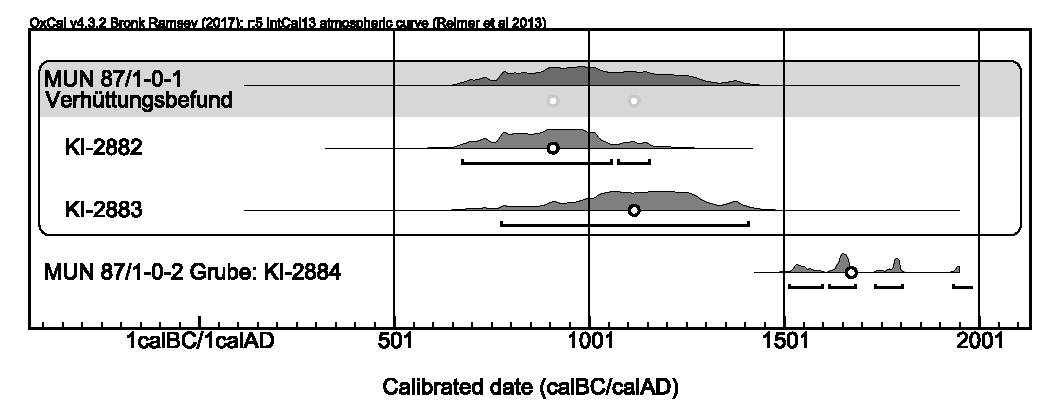
\includegraphics[width = .75\textwidth]{fig/MUN87_1_14C_sum.pdf}
		\captionof{figure}{MUN~87/1: Kalibrierung der Radiokohlenstoffdatierungen.}
		\label{fig:MUN87-1_14C-Kalibration}
	\end{minipage}
\end{figure*}

\begin{figure*}[p]
	\centering
	\begin{subfigure}{\columnwidth}	
		\centering
		\includegraphics[height = .4\textheight]{fig/MUN87-1-0-1_SchlackeOrganik.jpg}
		\caption{MUN~87/1-0-1: Grünliche Verhüttungsschlacken hoher Viskosität (Typ~2b) mit Pflanzenabdrücken (Fotos: D. Seidensticker, 2014).}
		\label{fig:MUN87-1_SchlackeOrganik}
	\end{subfigure}\hfill
	\begin{subfigure}{\columnwidth}
		\centering
		\includegraphics[height = .4\textheight]{fig/MUN87-1-0-2-6_Ofenwand.jpg}
		\caption{MUN~87/1-0-2: Ofen"-wand-Frag"-ment aus Abtrag 6 (0,8--0,9\,m unter der Oberfläche; Fotos: D. Seidensticker, 2014).}
		\label{fig:MUN87-1_Ofenwand}
	\end{subfigure}
	\caption{MUN~87/1: Sonstige Funde.}
\end{figure*}

\paragraph{Sonstige Funde}\hspace{-.5em}|\hspace{.5em}%
Neben der Keramik bilden Schlacken die zweithäufigste Fundgattung in beiden Befunden. Das Gros der insgesamt etwa 7,5\,kg Schlacke wurde im Verhüttungsbefund (MUN~87/1-0-1) gefunden (Abb.~\ref{fig:MUN87-1_VerteilungFunde}). Etwa 78\,\% der Schlacken sind auffällig grün gefärbte Fließschlacken hoher Viskosität vom Typ 2b (Abb.~\ref{fig:MUN87-12_Schlacken}). In der benachbarten Grube (MUN~87/1-0-2) fanden sich nur knapp etwa 500\,g Schlacke und es dominieren kantige Verhüttungsschlacken geringer Viskosität (Typ~4a).\footnote{In beiden Befunden finden sich auch grünliche Varianten der kantigen Verhüttungsschlacke geringer Viskosität.} Eine Auffälligkeit der Schlacken aus dem Verhüttungsbefund (MUN~87/1-0-1) sind regelhaft zu beobachtende Pflanzenabdrücke (Abb.~\ref{fig:MUN87-1_SchlackeOrganik}).

Das Fundinventar umfasst auch etwa 1,5\,kg gebrannten Lehm, der als potenzielle Ofenwandung interpretiert werden kann. Die noch bis etwa faustgroßen Brocken bestehen aus einem grob gemagerten Ton. Während eine der Seiten häufig rötlich gebrannt ist, ist die gegenüber liegende Seite schwarz verfärbt (Abb.~\ref{fig:MUN87-1_Ofenwand}).

\paragraph{Datierung}\hspace{-.5em}|\hspace{.5em}%
Aus den beiden in der Grabung MUN~87/1 erfassten Befunden stammen zusammen drei Radiokohlenstoffdatierungen (Tab.~\ref{tab:MUN87-1_14C-Daten}, Abb.~\ref{fig:MUN87-1_14C-Kalibration}). Auffällig ist der deutliche Unterschied zwischen zwei, das 7.--14.~Jh. n.~Chr. abdeckende Datierungen an Holzkohlen aus dem Verhüttungsbefund (KI-2882, KI-2883) und einer in das 16.--20.~Jh. n.~Chr. datierten Probe aus der Grube (KI-2884). Um ausreichend Material für eine konventionelle Radiokohlenstoffdatierung zu erhalten, wurden für eine der beiden Datierungen aus dem Verhüttungsbefund (KI-2882) Material von zwei Proben kombiniert. Diese \textit{bulk}-Probe lieferte das älteste Datum, überlappt sich in der Kalibration aber mit der zweiten Datierung aus dem Befund. 

\paragraph{Interpretation}\hspace{-.5em}|\hspace{.5em}%
Die Grabung MUN~87/1 erfasste einen aus zwei Bereichen bestehenden Komplex. Mit Blick auf die zeitliche Einordnung ergab die Auswertung einige widersprüchliche Befunde: die stratigrafische Relation der beiden Bereiche wurde durch das Zurückverlegen des Nordprofils im Schnittkastens von MUN~87/1-0-2 erfasst. Das Profil zeigt, dass der Verhüttungsbefund (MUN~87/1-0-1) jünger sein müsste als die Grube (MUN~87/1-0-2; Abb.~\ref{fig:MUN87-1_3Pl_T40Profil_C}). Jedoch muss beachtet werden, das dieser Befund lediglich in einem sehr begrenzten Bereich erfasst werden konnte.

Andererseits legen die vorliegenden drei Radiokohlenstoffdatierungen eine genau umgedrehte chronologische Position nahe. Die Holzkohlen aus dem Verhüttungsbefund sind deutlich älter als die Probe aus der Grube (Abb.~\ref{fig:MUN87-1_14C-Kalibration}). Dass sich die beiden Radiokohlenstoffdatierungen aus dem Verhüttungsbefund (MUN~87/1-0-1) nach der Kalibrierung nahezu exakt überschneiden, ist ein Indiz für die zeitliche Geschlossenheit der in dem kleinen Ofen gefundenen Holzkohlen.

Die Auswertung der Funde konnte nur bedingt Indizien für die Chronologie des Befundes beisteuern. Die wenige Keramik aus dem Verhüttungsbefund weist zwar Merkmale auf, die für eine ältere Zeitstellung sprechen, jedoch muss angenommen werden, dass die Scherben als \textit{Altfunde} in die Verfüllung des Befundes gelangt sind. In der Grube fand sich ein homogenes Inventar auf Vertretern des Ebambe-Stils, die potenziell eher in rezente Zeiten datieren (Kap.~\ref{sec:EBA-Gr}).

Zusammenfassend können drei Hypothesen für die chronologische Position der durch die Grabung erfassten Befunde formuliert werden: Vor der aktuellen Quellenlage als am wahrscheinlichsten angesehen wird eine Variante, in der beide Befunde in subrezente bis rezente Zeit datieren, wie das Radiokohlenstoffdatum aus der Grube es nahelegt. Zudem würde diese Variante durch die rezente Beobachtung von Ebambe-Keramik in Boyenge am Unterlauf des \mbox{Likwala}-\mbox{aux}-\mbox{Herbes} gestützt (Fpl.~284; Abb.~\ref{fig:EBA_BoyengeE8702310}). In diesem Fall müsste das deutlich ältere Datum für die beiden Radiokohlenstoffdatierungen aus dem Verhüttungsbefund interpretiert werden. Eine Möglichkeit dieses Umstandes könnte in einer potenziellen Nutzung von altem Holz für die Verhüttung liegen. Auch wäre es möglich, dass ältere, im direkten Umfeld aufgeschlossene Holzkohlen zusammen mit den Schlacken und wenigen Keramikscherben in die Verfüllung des kleinen Ofens gelangten.

Alternativ könnten beide Befunde auch in das 7.--14.~Jh. n.~Chr. datieren, wie die beiden Radiokohlenstoffdatierungen aus dem Verhüttungsbefund andeuten. Dies würde allerdings bedeuten, dass die analysierte Probe aus der Grube nicht das korrekte Alter des Befundes widerspiegelt und potenziell kontaminiert ist. Dieser Umstand ist in so fern nur bedingt zu akzeptieren, da die Probe aus einer Tiefe von etwas mehr als 0,5\,m unter der heutigen Oberfläche entnommen wurde.\footnote{Eine eher ältere chronologische Position vor allem der Ebambe-Keramik legt der Verhüttungsbefund in Pikunda am \mbox{Sangha} (Kat.-Nr.~10) nahe. Die Radiokohlenstoffdatierung aus diesem Befund fällt in das 11.--13.~Jh. n.~Chr. Zum Fundgut zählt auch eine GE, die der Ebambe-Gruppe zugerechnet werden kann. Leider fehlt die Grabungsdokumentation zu diesem Befund, wodurch der Zusammenhang zwischen dem Befund, der Probennahmestelle für Radiokohlenstoffdatierung und dem Bereich, in dem die GE gefunden wurde, nicht diskutiert werden kann (siehe Kap.~\ref{sec:EBA-Gr}).}

Es könnte aber auch keine zeitliche Kongruenz zwischen den beiden Befundteilen bestehen. Unter Akzeptanz, dass die Radiokohlenstoffdatierungen das Alter der jeweiligen Bereiche korrekt wiedergeben, müsste eine Erklärung für die stratigraphische Beobachtung gefunden werden, nach der der Ofen jünger als die Grube ist (Abb.~\ref{fig:MUN87-1_3Pl_T40Profil_C}). Nur unter Auflösung dieses Befundes ließe sich der Verhüttungsbefund in das 7.--14.~Jh. n.~Chr. datieren, während die Grube deutlich später angelegt wurde. Ein solches Szenario könnte zumindest erklären, warum sich in der Grube so viel weniger Schlacken fanden und bei der Grabung kein funktionaler Zusammenhang zwischen den beiden Teilen erfasst wurde.\footnote{Im Vergleich zum Verhüttungsbefund aus Pikunda am \mbox{Sangha} (Kat.-Nr.~10) fällt auf, dass der Befund in Munda keinen dezidierten Schlackenabfluss vom Verhüttungsbefund (MUN~87/1-0-1) in eine Schlackengrube (MUN~87/1-0-2) aufweist.}

Eine zweifelsfreie Rekonstruktion aller Prozesse, die zu dem durch die Grabung erschlossenen Befund geführt haben, ist nicht möglich. Es muss davon ausgegangen werden, dass der Ofen (\mbox{MUN~87/1-0-1}) im Anschluss an den Verhüttungsprozess ausgeräumt wurde. Andererseits zeigen das homogene Fundinventar und die teilweise vollständigen, auf der Seite oder Mündung liegend deponierten Gefäße in der Grube (\mbox{MUN~87/1-0-2}) eine zügige Verfüllung dieses Bereiches an.